\documentclass[openany, oneside]{book}
\usepackage[fontset=none]{ctex}
\usepackage{graphicx} % Required for inserting images
\usepackage{amsfonts, amsmath, amssymb, amsthm, mathtools}
\usepackage{float}
\usepackage{subfig}
\usepackage{color}
\usepackage{hyperref}
\usepackage[bottom=1in]{geometry}
\usepackage{tikz}
\usetikzlibrary{arrows, positioning}
\usepackage[ruled,linesnumbered,noend]{algorithm2e}
\usepackage[style=authoryear,maxbibnames=20,uniquename=false]{biblatex}
\usepackage{fancyhdr}


\setCJKmainfont[ItalicFont=FandolKai]{FandolSong}
\setCJKsansfont{FandolHei}
\setCJKmonofont{FandolKai}

\pagestyle{fancy}

\renewcommand{\headrulewidth}{0pt}

\fancyhf{} 
\fancyhead[L]{}
\fancyhead[C]{}
\fancyhead[R]{\thepage}

\newtheorem{remark}{备注}[section]
\newtheorem{theorem}{定理}[section]
\newtheorem{claim}{断言}[section]
\newtheorem{lemma}{引理}[section]
\newtheorem{corollary}{推论}[section]

\newtheorem*{remark*}{备注}
\newtheorem*{theorem*}{定理}
\newtheorem*{claim*}{断言}
\newtheorem*{lemma*}{引理}
\newtheorem*{corollary*}{推论}

\hypersetup{hidelinks}


\title{CS229 课程讲义}
\author{Andrew Ng (吴恩达) and Tengyu Ma (马腾宇)}
\date{由 \href{https://github.com/Na-moe/CS229_CN}{Namoe} 翻译\\June 2025}

\addbibresource{ref.bib}

\begin{document}

\maketitle

\begingroup
\fancyhead[L]{\textit{CS229 课程讲义}}
\fancyhead[C]{}
\fancyhead[R]{\thepage}
\tableofcontents
\clearpage
\endgroup

\part{监督学习}

不妨先从监督学习的几个例子谈起。假设有一个记录了俄勒冈州波特兰市 47 套房屋的居住面积和价格的数据集:

\begin{table}[h]
    \centering
    \begin{tabular}{c|c}
        居住面积 (平方英尺) & 价格 (1000\$) \\
        \hline
        2104 & 400 \\
        1600 & 330 \\
        2400 & 369 \\
        1416 & 232 \\
        3000 & 540 \\
        $\vdots$ & $\vdots$
    \end{tabular}
    \label{tab:house_example}
\end{table}

将这些数据绘制出来:

\begin{figure}[H]
    \centering
    \includegraphics[width=0.5\linewidth]{figs/house_dataset_plot1.pdf}
\end{figure}

有了这些数据之后,该怎样根据波特兰其他房屋的居住面积来预测其价格呢?

为了后续使用的方便,在这里做如下约定。约定用 $x^{(i)}$ 表示“输入”变量(示例中是居住面积),也称作输入\textbf{特征 (features)};用 $y^{(i)}$ 表示要预测的“输出”或\textbf{目标 (target) }变量(价格)。一对 $(x^{(i)}, y^{(i)})$ 称为一个\textbf{训练样本 (training example)},而用于学习的数据集——由 $n$ 个训练样本组成的列表 $\{(x^{(i)}, y^{(i)}); i = 1,...,n\}$——则称为\textbf{训练集 (training set)}。注意,此处的上标“$i$”仅表示训练集中的索引,而不表示指数运算。此外,用 $\mathcal{X}$ 表示输入的取值空间,$\mathcal{Y}$ 表示输出的取值空间。在本例中,有 $\mathcal{X} = \mathcal{Y} = \mathbb{R}$。

监督学习问题可以更加形式化地表述为:给定一个训练集,目标是学习一个函数 $h: \mathcal{X} \mapsto \mathcal{Y}$,该函数能够对输入 $x$ 进行预测,使其输出 $h(x)$ 与“很好地”预测相应的真实值 $y$。出于历史原因,函数 $h$ 被称为 \textbf{假设 (hypothesis)}。整个过程如下图所示:

\begin{figure}[H]
\centering
\begin{tikzpicture}[node distance=2cm, auto]
    \node [rounded corners=1mm, rectangle, align=center, draw] (training) {训练集};
    \node [rounded corners=1mm, rectangle, align=center, draw, below of=training] (learning) {学习算法};
    \node [rounded corners=1mm, rectangle, align=center, draw, below of=learning] (h) {$h$};
    \node [left of=h, label={[align=center]below:\footnotesize (房屋居住面积)}] (x) {$x$};
    \node [right of=h, label={[align=center]below:\footnotesize (房屋预测价格)}] (y) {预测值 $y$};

    \path [->, draw] (training) -- (learning);
    \path [->, draw] (learning) -- (h);
    \path [->, draw] (x) -- (h);
    \path [->, draw] (h) -- (y);
\end{tikzpicture}
\end{figure}

当预测的目标变量是连续值时(例如预测房价),称这类学习问题为\textbf{回归 (regression)} 问题。当 $y$ 只能取有限个离散值时(例如根据居住面积预测住宅是房屋还是公寓),则称为\textbf{分类 (classification)} 问题。

\input{part1_supervised_learning/chapter1_linear_regression}

\input{part1_supervised_learning/chapter2_classification_and_logistic_regression}

\input{part1_supervised_learning/chapter3_generalized_linear_models}

\input{part1_supervised_learning/chapter4_generative_learning_algorithms}

\input{part1_supervised_learning/chapter5_kernel_methods}

\input{part1_supervised_learning/chapter6_support_vector_machines}
\part{深度学习}

\input{part2_deep_learning/chapter7_deep_learning}
\part{泛化与正则化}

\input{part3_generalization_and_regularization/chapter8_generalization}

\chapter{正则化与模型选择}\label{chapter:9}

\section{正则化}



\section{隐式正则化效果 (选读)}


\section{通过交叉验证选择模型}


\section{贝叶斯统计与正则化}
\part{无监督学习}

\chapter{聚类与 k-means 算法}

\chapter{EM 算法}

\chapter{主成分分析 (PCA)}

\chapter{独立成分分析 (ICA)}

\chapter{自监督学习与基础模型}
\part{强化学习与控制}

\chapter{强化学习}

现在开始学习强化学习和自适应控制。

监督学习中的算法试图使其输出模仿训练集中的标签 $y$。在这种设置下,对于每个输入 $x$,标签都给出了明确的“正确答案”。然而,对于许多序列决策和控制问题,很难为学习算法提供这种显式监督。例如,如果我们构建了一个四足机器人并试图对其进行编程以使其行走,那么我们其实不知道什么是使其行走的“正确”动作,因此也不知道如何为学习算法提供显式监督以供其模仿。

强化学习将转而为算法提供一个奖励函数,该函数指示学习智能体何时表现良好,何时表现不佳。在四足行走示例中,奖励函数可以对机器人向前移动给予正奖励,而对向后移动或摔倒给予负奖励。然后,学习算法的任务就是随着时间推移确定如何选择动作以获得高奖励。

强化学习已成功应用于各种领域,包括自主直升机飞行、机器人腿部运动、蜂窝网络路由、营销策略选择、工厂控制和高效网页索引。对强化学习的研究将从定义\textbf{马尔可夫决策过程 (Markov decision processess, MDP)} 开始,它提供了表述强化学习问题的一般化形式化框架。

\section{马尔可夫决策过程}

马尔可夫决策过程是一个元组 $(S, A, \{P_{s a}\}, \gamma, R)$,其中:
\begin{itemize}
    \item $S$ 是一个\textbf{状态 (states)} 集合。(例如,在自主直升机飞行中,$S$ 可以是直升机所有可能的位置和方向的集合。)
    \item $A$ 是一个\textbf{动作 (actions)} 集合。(例如,可以推动直升机控制杆的所有可能方向的集合。)
    \item $P_{sa}$ 是状态转移概率 (state transition probabilities)。对于每个状态 $s \in S$ 和动作 $a \in A$, $P_{sa}$ 是状态空间上的一个分布。稍后会详细介绍,但简而言之,$P_{sa}$ 给出了如果在状态 $s$ 采取动作 $a$ 后将转移到哪些状态的分布。
    \item $\gamma \in [0, 1]$ 称为\textbf{折扣因子 (discount factor)}。
    \item $R: S \times A \mapsto \mathbb{R}$ 是\textbf{奖励函数 (reward function)}。(奖励有时也写成仅关于状态 $S$ 的函数,在这种情况下有 $R: S \mapsto \mathbb{R}$)。
\end{itemize}
MDP 的动态过程如下:我们从某个状态 $s_0$ 开始,然后在 MDP 中选择一个动作 $a_0 \in A$ 执行。然后 MDP 的状态随机转移到某个后继状态 $s_1$,根据 $s_1 \sim P_{s_0 a_0}$ 抽取。然后选择另一个动作 $a_1$。由于这个动作,状态再次转移,现在转移到某个 $s_2 \sim P_{s_1 a_1}$,依此类推。可以将这个过程表示为:
\[
    s_0 \xrightarrow{a_0} s_1 \xrightarrow{a_1} s_2 \xrightarrow{a_2} s_3 \xrightarrow{a_3} \dots
\]

以动作序列 $a_0, a_1, \dots$ 遍历状态序列 $s_0, s_1, \dots$ 后,总收益由下式给出
\[
    R(s_0, a_0) + \gamma R(s_1, a_1) + \gamma^2 R(s_2, a_2) + \dots.
\]
或者,将奖励写成仅关于状态的函数时,则变为
\[
    R(s_0) + \gamma R(s_1) + \gamma^2 R(s_2) + \dots.
\]
在大部分推导中,将使用更简单的状态奖励 $R(s)$,尽管推广到状态-动作奖励 $R(s, a)$ 也不会有特别的困难。

在强化学习中,目标是随着时间推移选择动作以最大化总收益的期望值:
\[
    \text{E}\left[R(s_0) + \gamma R(s_1) + \gamma^2 R(s_2) + \dots\right]
\]
注意,时间步 $t$ 的奖励被 $\gamma^t$ \textbf{折扣 (discount)}。因此,为了使这个期望值最大化,希望尽快累积正奖励(并尽可能推迟负奖励)。在经济应用中,如果 $R(\cdot)$ 代表赚取的金额,那么 $\gamma$ 也有一个自然的利率解释(今天的一美元比明天的一美元更值钱)。

\textbf{策略 (policy)} 是一个函数 $\pi: S \mapsto A$,它将状态映射到动作。当处于状态 $s$ 时,如果\textbf{执行 (executing)} 某个策略 $\pi$,则采取动作 $a = \pi(s)$。同时定义策略 $\pi$ 的\textbf{价值函数 (value function)} 为
\[
    V^\pi(s) = \text{E}\left[R(s_0) + \gamma R(s_1) + \gamma^2 R(s_2) + \dots \mid s_0 = s, \pi\right].
\]
$V^\pi(s)$ 表示从状态 $s$ 开始并按照策略 $\pi$ 采取动作所获得的折扣奖励的期望总和。\footnote{请注意,这里以 $\pi$ 为条件的写法并不完全正确,因为 $\pi$ 不是随机变量,但这在文献中是相当标准的用法。}

给定一个固定的策略 $\pi$,其价值函数 $V^\pi$ 满足\textbf{贝尔曼方程 (Bellman equation)}:
\[
    V^\pi(s) = R(s) + \gamma \sum_{s' \in S} P_{s\pi(s)}(s') V^\pi(s').
\]
这表明从状态 $s$ 开始的折扣奖励期望总和 $V^\pi(s)$ 由两部分组成:第一部分是从状态 $s$ 开始即刻获得的\textbf{即时奖励 (immediate reward)} $R(s)$;第二部分是未来折扣奖励的期望总和。仔细考察第二项,可以看到上面的求和项可以重写为 $\text{E}_{s' \sim P_{s\pi(s)}}[V^\pi(s')]$。这是从状态 $s'$ 开始的折扣奖励的期望总和,其中 $s'$ 的分布由 $P_{s\pi(s)}$ 给出,也就是在 MDP 中从状态 $s$ 执行第一个动作 $\pi(s)$ 后将到达的状态分布。因此,上面的第二项给出的是在 MDP 中执行第一步后获得的折扣奖励的期望总和。

贝尔曼方程可以有效地用于求解 $V^\pi$。具体来说,在一个有限状态 MDP ($|S| < \infty$) 中,可以为每个状态 $s$ 写出一个关于 $V^\pi(s)$ 的方程。这给出了 $|S|$ 个线性方程组,其中包含 $|S|$ 个变量(未知的 $V^\pi(s)$),可以有效地求解这些变量。

同样地,定义\textbf{最优价值函数 (optimal value function)} 为
\begin{equation}
    V^*(s) = \max_{\pi} V^\pi(s).
    \label{eq:15.1}
\end{equation}
换句话说,这是使用任何策略可以达到的最佳期望折扣奖励总和。对于最优价值函数,也有一个贝尔曼方程:
\begin{equation}
    V^*(s) = R(s) + \max_{a \in A} \gamma \sum_{s' \in S} P_{sa}(s') V^*(s').
    \label{eq:15.2}
\end{equation}
上面的第一项是即时奖励。第二项是在执行动作 $a$ 之后获得的期望未来折扣奖励总和在所有动作 $a$ 上的最大值。应该确保理解这个方程及其合理性。

同时定义策略 $\pi^*: S \mapsto A$ 如下:
\begin{equation}
    \pi^*(s) = \arg \max_{a \in A} \sum_{s' \in S} P_{sa}(s') V^*(s').
    \label{eq:15.3}
\end{equation}
注意,$\pi^*(s)$ 给出了在方程\eqref{eq:15.2}中的 "max" 中达到最大值的动作 $a$。

事实证明,对于每一个状态 $s$ 和每一个策略 $\pi$,有
\[
    V^*(s) = V^{\pi^*}(s) \ge V^\pi(s).
\]
第一个等号表示,对于每个状态 $s$,策略 $\pi^*$ 的价值函数 $V^{\pi^*}$ 都等于最优价值函数 $V^*$。此外,不等号表示 $\pi^*$ 的价值至少与任何其他策略的价值一样大。换句话说,方程 \eqref{eq:15.3} 所定义的 $\pi^*$ 是\textbf{最优策略 (optimal policy)}。

注意,$\pi^*$ 具有一个有趣的性质,即它是\textit{所有 (all)} 状态 $s$ 的最优策略。也就是说,不会是这样:从某个状态 $s$ 开始的最优策略,与从另一个状态 $s'$ 开始的最优策略不同。同一个策略 $\pi^*$ 在\textit{所有 (all)} 状态 $s$ 下都达到了方程 \eqref{eq:15.1} 的最大值。这意味着无论 MDP 的初始状态是什么,都可以使用相同的策略 $\pi^*$。

\section{价值迭代与策略迭代}\label{sec:15.2}

现在介绍两种求解有限状态 MDP 的高效算法。目前,只考虑具有有限状态空间和动作空间(即 $|S| < \infty, |A| < \infty$)的 MDP。在本节中,还假设已知状态转移概率 $\{P_{sa}\}$ 和奖励函数 $R$。

第一个算法是\textbf{价值迭代 (value iteration)},如下所示:

\vspace{0.5em}
\begin{algorithm}[H]
    \SetAlgoNoLine
    \label{algo:4}
    \caption{价值迭代}
    对于每个状态 $s$,初始化 $V(s) := 0$。\\
    \For{直到收敛}{
        对于每个状态,更新
        \begin{equation}\label{eq:15.4}
            V(s) := R(s) + \max_{a \in A} \gamma \sum_{s'} P_{sa}(s') V(s').
        \end{equation}
    }
\end{algorithm}

这个算法可以看作是重复使用贝尔曼方程\eqref{eq:15.2}来更新估计的价值函数。

算法的内循环中更新 $V(s)$ 的方式有两种方式。第一种是先计算每个状态 $s$ 的新 $V(s)$ 值,然后用新值覆盖所有旧值。这称为\textbf{同步 (synchronous)} 更新。在这种情况下,算法可以看作是实现了一个“贝尔曼备份算子”,它接收价值函数的当前估计,并将其映射到一个新的估计。(详请参阅习题集。)另一种方法是执行\textbf{异步 (asynchronous)} 更新。在这种情况下,可以按某种顺序逐个状态进行循环,每次更新一个值。

在同步或异步更新下,可以证明价值迭代会使 $V$ 收敛到 $V^*$。找到 $V^*$ 后,可以使用方程\eqref{eq:15.3}来找到最优策略。

除了价值迭代,还有另一种算法用于寻找 MDP 的最优策略。\textbf{策略迭代 (policy iteration)} 算法如下:

\vspace{0.5em}
\begin{algorithm}[H]
    \SetKwComment{Comment}{$\triangleright$\ }{}
    \SetAlgoNoLine
    \label{algo:5}
    \caption{策略迭代}
    随机初始化 $\pi$。\\
    \For{直到收敛}{
        令 $V := V^\pi.$ \Comment*[f]{通常用线性系统求解器处理}\\
        对于每个状态 $s$,令
        \begin{equation*}
            \pi(s) := \arg\max_{a \in A} \sum_{s'}P_{s a}(s')V(s').
        \end{equation*}
    }
\end{algorithm}

因此,内循环重复计算当前策略的价值函数,然后使用当前价值函数更新策略。(步骤 (b) 中找到的策略也称为关于 $V$ 的\textbf{贪婪策略 (greedy policy)}。)注意,步骤 (a) 可以通过求解贝尔曼方程来实现,如前所述,对于一个固定的策略,这仅仅是关于 $|S|$ 个变量的 $|S|$ 个线性方程组。
经过该算法的\textit{有限 (finite)} 次迭代后,$V$ 将收敛到 $V^*$,并且 $\pi$ 将收敛到 $\pi^*$。\footnote{注意,价值迭代无法在有限次迭代中达到精确的 $V^*$,但策略迭代可以使用精确的线性方程组求解器,因此可以精确收敛。这是因为当动作空间和策略空间是离散且有限时,一旦策略迭代中的策略达到最优策略,它将不再改变。另一方面,尽管价值迭代会收敛到 $V^*$,但学习到的价值函数中总是存在一些非零误差。}

价值迭代和策略迭代都是求解 MDP 的标准算法,目前对于哪种算法更好还没有普遍共识。对于小型 MDP,策略迭代通常非常快,并且在很少的迭代次数内收敛。然而,对于状态空间较大的 MDP,显式求解 $V^*$ 将涉及求解一个大型线性方程组,这可能会很困难(并且注意在策略迭代中需要多次求解线性方程组)。在这些问题中,价值迭代可能更受欢迎。因此,在实践中,价值迭代似乎比策略迭代更常用。关于价值迭代和策略迭代的比较和联系的更多讨论,请参阅第 \ref{sec:15.5} 节。

\section{学习 MDP 的模型}

到目前为止,所讨论的 MDP 和求解 MDP 的算法都假设已知状态转移概率和奖励。在许多现实问题中,我们无法直接获得状态转移概率和奖励,而是必须从数据中估计它们。(通常,状态空间 $S$、动作空间 $A$ 和折扣因子 $\gamma$ 是已知的。)例如,假设对于倒立摆问题(参见习题集 4),我们在 MDP 中进行了一些试验,过程如下:
\begin{align*}
    &s_0^{(1)} \xrightarrow{a_0^{(1)}} s_1^{(1)} \xrightarrow{a_1^{(1)}} s_2^{(1)} \xrightarrow{a_2^{(1)}} s_3^{(1)} \xrightarrow{a_3^{(1)}} \dots \\
    &s_0^{(2)} \xrightarrow{a_0^{(2)}} s_1^{(2)} \xrightarrow{a_1^{(2)}} s_2^{(2)} \xrightarrow{a_2^{(2)}} s_3^{(2)} \xrightarrow{a_3^{(2)}} \dots\\
    &\cdots
\end{align*}
这里,$s_i^{(j)}$ 是在第 $j$ 次试验的时刻 $i$ 时的状态,$a_i^{(j)}$ 是在该状态下采取的相应动作。在实践中,上述每一次试验可能会持续到 MDP 终止(例如,倒立摆问题中,摆杆倒下),或者可能运行很长但有限的时间步。

给定由多次试验组成的 MDP 中的这种“经验”,可以很容易地得出状态转移概率的最大似然估计:
\begin{equation}
    P_{sa}(s') = \frac{\text{在状态 $s$ 采取动作 $a$ 到达状态 $s'$ 的次数}}{\text{在状态 $s$ 采取动作 $a$ 的次数}}
    \label{eq:15.5}
\end{equation}
或者,如果上述比率是“0/0”——对应于之前从未在状态 $s$ 采取动作 $a$ 的情况——我们可以简单地将 $P_{sa}(s')$ 估计为 $1/|S|$。(即,将 $P_{sa}$ 估计为关于所有状态的均匀分布。)

注意,如果得到了更多经验(观察了更多试验),有一种有效的方法可以使用新的经验更新状态转移概率估计。具体来说,如果我们跟踪 \eqref{eq:15.5} 中分子和分母的计数,那么当观察更多试验时,可以简单地累加这些计数。计算这些计数的比率即可得到对 $P_{sa}$ 的估计。

使用类似的过程,如果 $R$ 未知,也可以将状态 $s$ 中预期即时奖励 $R(s)$ 的估计值取为在状态 $s$ 中观察到的平均奖励。

在学习了 MDP 的模型后,可以使用价值迭代或策略迭代来求解 MDP,使用估计的状态转移概率和奖励。例如,将模型学习和价值迭代结合起来,是学习具有未知状态转移概率的 MDP 的一种可能的算法:

\begin{enumerate}
    \item 随机初始化 $\pi$。
    \item 重复 \{
        \begin{enumerate}
            \item 在 MDP 中执行一定次数的 $\pi$,收集经验。
            \item 使用上述经验更新状态转移概率 $P_{sa}$ 的估计值(如果可行的话,也更新 $R$ 的估计值)。
            \item 根据估计的状态转移概率和奖励,使用价值迭代更新价值函数 $V$ 的估计值。
            \item 更新策略 $\pi$,使其成为关于 $V$ 的贪婪策略。
        \end{enumerate}
    \}
\end{enumerate}

注意到,对于该算法,有一个简单的优化可以使其运行得更快。具体来说,在算法的内层循环中,应用价值迭代时,如果不是将价值迭代初始化为 $V=0$,而是用算法前一次迭代中找到的解进行初始化,那么这将为价值迭代提供一个更好的起始点,并使其更快收敛。

\section{连续状态 MDP}

之前我们主要关注了有限状态数量的 MDP。现在我们将讨论可能具有无限状态数量的 MDP 的算法。例如,对于汽车,我们可以将状态表示为 $(x, y, \theta, \dot{x}, \dot{y}, \dot{\theta})$,其中包括其位置 $(x, y)$;方向 $\theta$;在 $x$ 和 $y$ 方向上的速度 $\dot{x}$ 和 $\dot{y}$;以及角速度 $\dot{\theta}$。因此,$S = \mathbb{R}^6$ 是一个无限状态集,因为汽车有无限多的可能位置和方向。\footnote{严格来说,$\theta$ 是一个方向,因此 $\theta$ 的范围写成 $\theta \in [-\pi, \pi)$ 比 $\theta \in \mathbb{R}$ 更合适;但对我们的目标而言,这种区别并不重要。} 类似地,在习题集 4 中的倒立摆具有状态 $(x, \theta, \dot{x}, \dot{\theta})$,其中 $\theta$ 是摆杆的角度。而一架在 3D 空间中飞行的直升机具有 $(x, y, z, \phi, \theta, \psi, \dot{x}, \dot{y}, \dot{z}, \dot{\phi}, \dot{\theta}, \dot{\psi})$ 形式的状态,其中横滚角 $\phi$、俯仰角 $\theta$ 和偏航角 $\psi$ 指定了直升机的 3D 方向。

在本节中,我们将考虑状态空间为 $S = \mathbb{R}^d$ 的情况,并描述解决此类 MDP 的方法。

\subsection{离散化}

解决连续状态 MDP 的最简单方法可能是离散化状态空间,然后使用之前描述的价值迭代或策略迭代等算法。

例如,对于 2D 状态 $(s_1, s_2)$,可以使用网格来离散化状态空间:

\begin{figure}[H]
    \centering
    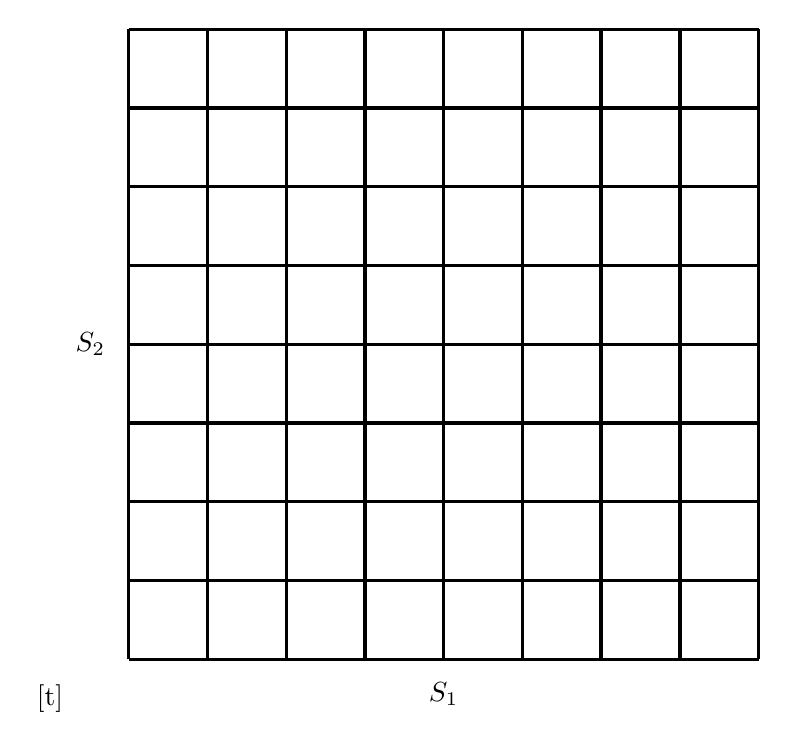
\begin{tikzpicture}
        \def\gridsize{8}
        \draw[step=1, very thick, black] (0,0) grid (\gridsize, \gridsize);
        \node[below=5pt] at (\gridsize/2, 0) {$S_1$};
        \node[left=5pt] at (0, \gridsize/2) {$S_2$};
        \node at (-1, -0.5) {[t]};
    \end{tikzpicture}
\end{figure}

这里,每个网格单元代表一个独立的离散状态 $\bar{s}$。然后,可以通过一个离散状态 MDP $(\bar{S}, A, \{P_{\bar{s}a}\}, \gamma, R)$ 来近似连续状态 MDP,其中 $\bar{S}$ 是离散状态的集合,$\{P_{\bar{s}a}\}$ 是离散状态上的状态转移概率。然后,可以使用价值迭代或策略迭代来解出离散状态 MDP $(\bar{S}, A, \{P_{\bar{s}a}\}, \gamma, R)$ 中的 $V^*(\bar{s})$ 和 $\pi^*(\bar{s})$。当实际系统处于某个连续值状态 $s \in S$ 并且需要选择一个动作来执行时,就计算相应的离散化状态 $\bar{s}$,并执行动作 $\pi^*(\bar{s})$。

这种离散化方法对于许多问题都能很好地工作。然而,它有两个缺点。首先,它对 $V^*$(以及 $\pi^*$)使用了相当简单的表示。具体来说,它假设价值函数在每个离散化区间上取一个常数值(即,价值函数在每个网格单元中是分段常数)。

为了更好地理解这种表示的局限性,考虑一个\textit{监督学习 (supervised learning)} 问题,将函数拟合到这个数据集:

\begin{figure}[H]
    \centering
    \includegraphics[width=0.6\textwidth]{figs/rl_dataset.png}
\end{figure}

显然,线性回归可以很好地拟合这个数据集,然而,如果对 x 轴离散化,并使用在每个离散区间内为分段常数的表示,那么我们对数据的拟合将如下所示:

\begin{figure}[H]
    \centering
    \includegraphics[width=0.6\textwidth]{figs/rl_dataset_discrete.png}
\end{figure}

这种分段常数表示对于许多平滑函数来说并不是一个好的表示。它导致输入上的平滑性很差,并且在不同网格单元之间没有泛化能力。使用这种表示,我们需要非常精细的离散化(非常小的网格单元)才能获得良好的近似。

这种表示的第二个缺点被称为\textbf{维度诅咒 (curse of dimensionality)}。假设 $S = \mathbb{R}^d$,并且我们将状态的 $d$ 个维度中的每一个都离散化为 $k$ 个值。那么我们拥有的离散状态总数为 $k^d$。这在状态空间维度 $d$ 中呈指数级增长,因此不适用于大型问题。例如,对于一个 10 维状态,如果我们将每个状态变量离散化为 100 个值,我们将有 $100^{10} = 10^{20}$ 个离散状态,这对于现代计算机来说也大到无法表示。

根据经验,离散化通常对于 1 维和 2 维问题非常有效(而且简单且快速实现)。也许用一些取巧的办法,并在选择离散化方法时谨慎一些,它也能适用于 4 维状态的问题。如果你非常聪明且幸运,甚至可能让它适用于某些 6 维问题。但它很少适用于更高维度的问题。

\subsection{价值函数近似}

我们现在介绍一种在连续状态 MDP 中寻找策略的替代方法,即直接近似 $V^*$,而无需诉诸离散化。这种方法被称为价值函数近似,且已成功应用于许多强化学习问题。

\subsubsection*{使用模型或模拟器}

为了开发值函数近似算法,我们将假设我们拥有一个用于 MDP 的\textbf{模型 (model)} 或\textbf{模拟器 (simulator)}。非正式地,模拟器是一个黑盒,它接收任何(连续值)状态 $s_t$ 和动作 $a_t$ 作为输入,并根据状态转移概率 $P_{s_t a_t}$ 输出下一个状态 $s_{t+1}$ 的采样。

\begin{figure}[H]
    \centering
    \includegraphics[width=0.5\textwidth]{figs/simulator.pdf}
\end{figure}

获取此类模型有多种方法。一种是使用物理模拟。例如,习题集 4 中倒立摆的模拟器是通过使用物理定律计算在给定当前状态 $t$ 和所采取的动作 $a$ 的情况下,小车/杆在时间 $t+1$ 的位置和方向来获得的,前提是已知系统的所有参数,例如杆的长度、杆的质量等。或者,也可以使用现成的物理模拟软件包,该软件包将机械系统的完整物理描述、当前状态 $s_t$ 和动作 $a_t$ 作为输入,并在未来一小段时间内计算出系统的状态 $s_{t+1}$。\footnote{Open Dynamics Engine (\url{http://www.ode.com}) 是一个免费/开源的物理模拟器示例,可用于模拟倒立摆等系统,并且在强化学习研究人员中一直是一个受欢迎的选择。}

获取模型的另一种方法是从 MDP 中收集的数据中学习一个模型。例如,假设执行 $n$ 次\textbf{试验 (trials)},每次试验重复在 MDP 中采取动作,且持续 $T$ 个时间步。可以随机选择动作、执行某些特定策略或通过其他方式选择动作。然后,将观察到 $n$ 个状态序列,如下所示:
\begin{align*}
    &s_0^{(1)} \xrightarrow{a_0^{(1)}} s_1^{(1)} \xrightarrow{a_1^{(1)}} s_2^{(1)} \xrightarrow{a_2^{(1)}} \dots \xrightarrow{a_{T-1}^{(1)}} s_T^{(1)} \\
    &s_0^{(2)} \xrightarrow{a_0^{(2)}} s_1^{(2)} \xrightarrow{a_1^{(2)}} s_2^{(2)} \xrightarrow{a_2^{(2)}} \dots \xrightarrow{a_{T-1}^{(2)}} s_T^{(2)} \\
    &\dots \\
    &s_0^{(n)} \xrightarrow{a_0^{(n)}} s_1^{(n)} \xrightarrow{a_1^{(n)}} s_2^{(n)} \xrightarrow{a_2^{(n)}} \dots \xrightarrow{a_{T-1}^{(n)}} s_T^{(n)}
\end{align*}
然后,可以应用学习算法来预测 $s_{t+1}$ 作为 $s_t$ 和 $a_t$ 的函数。

例如,可以选择学习一个如下形式的线性模型:
\begin{equation}
    s_{t+1} = As_t + Ba_t,
    \label{eq:15.6}
\end{equation}
使用类似于线性回归的算法。这里,模型的参数是矩阵 $A$ 和 $B$,并且可以通过从 $n$ 次试验中收集的数据来估计它们:
\[
    \underset{A,B}{\arg \min} \sum_{i=1}^n \sum_{t=0}^{T-1} \left\| s_{t+1}^{(i)} - (As_t^{(i)} + Ba_t^{(i)}) \right\|^2.
\]

也可以使用其他损失函数来学习模型。例如,最近 \cite{luo2018algorithmic} 的工作发现,使用 $\left\| \cdot \right\|_2$ 范数(不带平方)在某些情况下可能有所帮助。

在学习了 $A$ 和 $B$ 之后,一个选项是构建一个\textbf{确定性 (deterministic)} 模型,其中给定输入 $s_t$ 和 $a_t$,输出 $s_{t+1}$ 被精确确定。具体来说,总是根据公式 \eqref{eq:15.6} 计算 $s_{t+1}$。或者,也可以构建一个\textbf{随机 (stochastic)} 模型,其中 $s_{t+1}$ 是输入的随机函数,通过将其建模为:
\[
    s_{t+1} = As_t + Ba_t + \epsilon_t,
\]
其中 $\epsilon_t$ 是一个噪声项,通常建模为 $\epsilon_t \sim \mathcal{N}(0, \Sigma)$。(协方差矩阵 $\Sigma$ 也可以以直接的方式从数据中估计。)

这里将下一个状态 $s_{t+1}$ 写成当前状态和动作的线性函数;当然,这也可以是非线性函数。具体来说,可以学习一个模型 $s_{t+1} = A\phi_s(s_t) + B\phi_a(a_t)$,其中 $\phi_s$ 和 $\phi_a$ 是状态和动作的一些非线性特征映射。或者,也可以使用非线性学习算法,例如局部加权线性回归,来估计 $s_{t+1}$ 作为 $s_t$ 和 $a_t$ 的函数。这些方法都可以用来构建 MDP 的确定性或随机模拟器。

\subsubsection*{拟合价值迭代}

现在介绍用于近似连续状态 MDP 价值函数的\textbf{拟合价值迭代 (fitted value iteration)} 算法。在下文中,我们将假设问题具有连续状态空间 $S = \mathbb{R}^d$,但动作空间 $A$ 较小且离散。\footnote{在实践中,大多数 MDP 的动作空间远小于状态空间。例如,汽车状态空间有 6 维而动作空间则是 2 维(转向和速度控制);倒立摆状态空间有 4 维而动作空间只有 1 维;直升机则是 12 维状态空间和 4 维动作空间。因此,离散化动作空间通常比离散化状态空间的问题要小得多。}

回顾一下,价值迭代执行以下更新:
\begin{align}
    V(s) &:= R(s) + \gamma \max_a \int_{s'} P_{sa}(s')V(s')ds' \label{eq:15.7} \\
    &= R(s) + \gamma \max_a \mathrm{E}_{s' \sim P_{sa}} [V(s')] \label{eq:15.8}
\end{align}
(在第 \ref{sec:15.2} 节中,价值迭代更新写为 $V(s) := R(s) + \gamma \max_a \sum_{s'} P_{sa}(s')V(s')$ 而不是状态上的积分;新的符号反映了现在正在处理连续状态而不是离散状态。)

拟合价值迭代的主要思想是,在有限样本状态 $s^{(1)}, \dots, s^{(n)}$ 上近似地执行此步骤。具体来说,下面使用监督学习算法——线性回归——来近似状态的价值函数,作为状态的线性或非线性函数:
\[
    V(s) = \theta^T \phi(s).
\]
这里,$\phi$ 是状态的某种适当的特征映射。

对于具有的有限样本 $n$ 个状态中的每个状态 $s$,拟合价值迭代将首先计算一个量 $y^{(i)}$,是 $R(s) + \gamma \max_a \mathrm{E}_{s' \sim P_{sa}} [V(s')]$ 的近似(公式 \eqref{eq:15.8} 的右侧)。然后将应用监督学习算法,尝试使 $V(s)$ 接近 $R(s) + \gamma \max_a \mathrm{E}_{s' \sim P_{sa}} [V(s')]$(换句话说,尝试使 $V(s)$ 接近 $y^{(i)}$)。

详细来说,该算法如下:
\begin{enumerate}
    \item 随机采样 $n$ 个状态 $s^{(1)}, s^{(2)}, \cdots, s^{(n)} \in S$。
    \item 初始化 $\theta := 0$。
    \item 重复 \{
        \begin{itemize}
            \item[] 对于 $i = 1, \dots, n$ \{
                \begin{itemize}
                    \item[] 对于每个动作 $a \in A$ \{
                        \begin{itemize}
                            \item[] 采样 $s_1', \cdots, s_k' \sim P_{s^{(i)} a}$(使用某种 MDP 模型)。
                            \item[] 令 $q(a)=\frac1k \sum_{j=1}^{k} R(s^{(i)}) + \gamma V(s_j')$。
                            \item[] \qquad // 因此,$q(a)$ 是 $R(s^{i}) + \gamma \mathrm{E}_{s'\sim P_{s^{(i) a}}}[V(s')]$ 的估计值。
                        \end{itemize}

                    \}
                    \item[] 令 $y^{(i)} = \max_a q(a)$。
                    \item[] \qquad // 因此, $y^{(i)}$ 是 $R(s^{i}) + \gamma \max_a \mathrm{E}_{s'\sim P_{s^{(i) a}}}[V(s')]$ 的估计值。
                \end{itemize}
            \}
            \item[] // 原始的(用于离散状态的)价值迭代算法
            \item[] // 根据 $V(s^{(i)}) := y^{(i)}$ 更新价值函数。
            \item[] // 此算法则希望 $V(s^{(i)}) \approx y^{(i)}$
            \item[] // 可以使用监督学习(线性回归)达成这点。
            \item[] 令 $\theta := \arg\min_\theta \frac12 \sum_{i=1}^{n} \left(\theta^T \phi(s^{(i)}) - y^{(i)}\right)^2$。
        \end{itemize}
        
    \}
\end{enumerate}

如上所述,我们已经详细阐述了使用线性回归的拟合价值迭代算法,以使 $V(s^{(i)})$ 接近 $y^{(i)}$。算法的这一步骤完全类似于标准的监督学习(回归)问题,其中有一个训练集 $(x^{(1)}, y^{(1)}), (x^{(2)}, y^{(2)}), \dots, (x^{(n)}, y^{(n)})$,并且希望学习一个从 $x$ 到 $y$ 的函数;唯一的区别是这里 $s$ 扮演了 $x$ 的角色。尽管上面的描述使用了线性回归,但显然也可以使用其他回归算法(例如局部加权线性回归)。

与离散状态集上的价值迭代不同,拟合价值迭代不能被证明总是收敛的。然而,它在实践中通常能收敛(或近似收敛),并且对许多问题都表现良好。还需要注意的是,如果使用 MDP 的确定性模拟器/模型,那么可以通过在算法中设置 $k=1$ 来简化拟合价值迭代。这是因为公式 \eqref{eq:15.8} 中的期望变为确定性分布上的期望,因此一个单一的样本就足以精确计算该期望。否则,在上述算法中,需要抽取 $k$ 个样本并取平均值来近似该期望(参见算法伪代码中 $q(a)$ 的定义)。

最后,拟合价值迭代输出 $V$ 作为 $V^*$ 的近似。这隐式地定义了我们的策略。具体来说,当系统处于某个状态 $s$,需要选择一个动作时,我们希望选择以下动作:
\begin{equation}
    \arg \max_a \mathrm{E}_{s' \sim P_{sa}} [V(s')] \label{eq:15.9}
\end{equation}
计算/近似此过程类似于拟合价值迭代的内循环,其中对于每个动作,我们从 $P_{sa}$ 中采样 $s'_1, \dots, s'_k$ 来近似期望。(同样,如果模拟器是确定性的,我们可以设置 $k=1$。)

在实践中,通常还有其他方法来近似此步骤。例如,一个非常常见的情况是模拟器具有 $s_{t+1} = f(s_t, a_t) + \epsilon_t$ 的形式,其中 $f$ 是状态的某个确定性函数(例如 $f(s_t, a_t) = As_t + Ba_t$),$\epsilon_t$ 是零均值高斯噪声。在这种情况下,我们可以通过以下方式选择动作:
\[
    \arg \max_a V(f(s, a)).
\]
换句话说,这里是设置 $\epsilon_t = 0$(即,忽略模拟器中的噪声),并设置 $k=1$。等效地,这可以从公式 \eqref{eq:15.9} 使用以下近似导出:
\begin{align}
    \mathrm{E}_{s'}[V(s')] &\approx V(\mathrm{E}_{s'}[s']) \label{eq:15.10} \\
    &= V(f(s, a)), \label{eq:15.11}
\end{align}
其中期望是关于随机变量 $s' \sim P_{sa}$ 的。只要噪声项 $\epsilon_t$ 很小,这通常是一个合理的近似。

然而,对于那些不适合这种近似的问题,为了近似上述期望,需要使用模型对 $k|A|$ 个状态进行采样,这在计算上可能非常昂贵。

\section{策略与价值的联系 (选读)}\label{sec:15.5}

\vspace{0.5em}
\begin{algorithm}[H]
    \SetKwComment{Comment}{$\triangleright$\ }{}
    \SetAlgoNoLine
    \label{algo:6}
    \caption{策略迭代的变体}
    \textbf{过程} VE($\pi$, k) \Comment*[f]{用于评估 $V^\pi$}\\
    \quad 选项 1:初始化 $V := 0$;选项 2:使用主算法的当前 $V$ 进行初始化。\\
    \quad \For{$i=0$ \KwTo $k-1$}{
        \quad 对于每个状态 $s$,更新
        \begin{equation}
            V(s) := R(s) + \gamma \sum_{s'} P_{s \pi(s)}(s')V(s').\label{eq:15.12}
        \end{equation}
    }
    \textbf{返回} $V$

    \ \\
    \textbf{输入}\ 超参数 $k$。\\
    随机初始化 $\pi$。\\
    \For{直到收敛}{
        令 $V := VE(\pi, k).$\\
        对于每个状态 $s$,令
        \begin{equation}
            \pi(s) := \arg\max_{a \in A} \sum_{s'}P_{s a}(s')V(s').\label{eq:15.13}
        \end{equation}
    }
\end{algorithm}

在策略迭代算法 \ref{algo:5} 的第 3 行,通常用线性系统求解器来计算 $V^\pi$。或者也可以使用迭代贝尔曼更新来评估 $V^\pi$,这类似于价值迭代,如算法 \ref{algo:6} 中过程 VE($\cdot$) 的第 1 行所示。如果我们在过程 VE 的第 2 行中选择选项 1,那么过程 VE 与价值迭代(算法 \ref{algo:4})的不同之处在其第 4 行:过程 VE 用 $\pi$ 中的动作,而价值迭代则使用贪婪动作。

用过程 VE 可以构建算法 \ref{algo:6},它是策略迭代的一种变体,作为连接策略迭代和价值迭代的中间算法。这里我们在 VE 中选用选项 2,以最大化重用之前所学的知识。可以验证,如果取 $k=1$ 并在算法 \ref{algo:6} 的第 2 行中选用选项 2,那么算法 \ref{algo:6} 在语义上等同于价值迭代(算法 \ref{algo:4})。换句话说,算法 \ref{algo:6} 和价值迭代交错更新 \eqref{eq:15.13} 和 \eqref{eq:15.12}。算法 \ref{algo:6} 在更新 $k$ 步 \eqref{eq:15.12} 和一步 \eqref{eq:15.13} 之间交替,而价值迭代在更新一步 \eqref{eq:15.12} 和一步 \eqref{eq:15.13} 之间交替。因此,算法 \ref{algo:6} 通常不会比价值迭代更快,因为假设更新 \eqref{eq:15.12} 和 \eqref{eq:15.13} 效用和耗时相同,那么更新频率的最佳平衡可能只是 $k=1$ 或 $k \approx 1$。

另一方面,如果更新 $k$ 步 \eqref{eq:15.12} 可以比更新一步 \eqref{eq:15.12} $k$ 次快得多,那么多求几步 \eqref{eq:15.12} 可能有用。这就是策略迭代所利用的——线性系统求解器求解 $k=\infty$ 的 VE 比求解较大的 $k$ 的 VE 会快得多。反之,如果不存在这种加速效果,例如当状态空间很大且线性系统求解器也不快时,价值迭代更可取。

\chapter{LQR, DDP 与 LQG}

\section{有限时间范围的 MDP}\label{sec:16.1}

第15章中定义了马尔可夫决策过程,并讨论了简化设置下的价值迭代/策略迭代。具体而言,引入了定义最优策略 $\pi^*$ 的最优价值函数 $V^*$ 的\textbf{最优贝尔曼方程 (optimal Bellman equation)}。
\[
    V^*(s) = R(s) + \max_{a \in A}\gamma \sum_{s' \in S} P_{sa}(s')V^*(s')
\]

回想一下,从最优价值函数中能恢复最优策略$\pi^*$,如下所示:
\[
    \pi^*(s) = \operatorname*{argmax}_{a \in A} \sum_{s' \in S} P_{sa}(s')V^*(s')
\]

在本章中,将采用更一般的设置:
\begin{enumerate}
    \item 为了同时适用于离散和连续的情况。因此,将使用
    \begin{align*}
        &\mathbb{E}_{s' \sim P_{sa}}[V^{\pi^*}(s')] \quad \text{而非} \\
        &\sum_{s' \in S} P_{sa}(s')V^{\pi^*}
    \end{align*}
    这意味着将取下一状态价值函数的期望。在离散情况下,可以将期望改写为对所有状态的求和。在连续情况下,可以将期望改写为对所有状态的积分。符号 $s' \sim P_{sa}$ 表示 $s'$ 是从分布 $P_{sa}$ 中采样的。
    \item  假设奖励同时取决于\textbf{状态和动作 (both states and actions)}。换句话说,$R: \mathcal{S} \times \mathcal{A} \to \mathbb{R}$。这意味着计算最优动作的先前机制变为
    \[
        \pi^*(s) = \underset{a \in \mathcal{A}}{\text{argmax}} \ R(s, a) + \gamma \mathbb{E}_{s' \sim P_{sa}} [V^{\pi^*}(s')]
    \]
    \item 不考虑无限时间范围的 MDP,而是假设有一个\textbf{有限时间范围的 MDP (finite horizon MDP)},定义为一个元组
    \[
        (\mathcal{S}, \mathcal{A}, P_{sa}, T, R)
    \]
    其中 $T > 0$ 是\textbf{时间范围 (time horizon)}(例如 $T=100$)。在这种设置下,对回报的定义将略有不同:
    \[
        R(s_0, a_0) + R(s_1, a_1) + \cdots + R(s_T, a_T)
    \]
    而不是(无限时间范围情况下的)
    \begin{align*}
        & R(s_0, a_0) + \gamma R(s_1, a_1) + \gamma^2 R(s_2, a_2) + \cdots
        & \sum_{t=0}^{\infty} R(s_t, a_t)\gamma^t
    \end{align*}
    \textit{折现因子 $\gamma$ 呢?(what happened to the discount factor $\gamma$?)} 请记住,引入 $\gamma$ (部分原因)是为了确保无限项求和是有限且良定义的。如果奖励以常数 $\bar{R}$ 为界,则回报是以下式为界的
    \[
        \left| \sum_{t=0}^{\infty} R(s_t)\gamma^t \right| \leq \bar{R} \sum_{t=0}^{\infty} \gamma^t
    \]
    发现这里是一个几何级数!在这里,由于回报是有限项求和,折现因子 $\gamma$ 不再是必需的。

    在这种新设置中,情况表现得相当不同。首先,最优策略 $\pi^*$ 可能是非平稳的,这意味着\textbf{它随时间变化 (it changes over time)}。换句话说,现在有
    \[
        \pi^{(t)}: \mathcal{S} \to \mathcal{A}
    \]
    其中上标 $(t)$ 表示时间步 $t$ 的策略。遵循策略 $\pi^{(t)}$ 的有限时间范围 MDP 的动态过程如下:从某个状态 $s_0$ 开始,根据时间步 0 的策略 $\pi^{(0)}(s_0)$ 采取某个动作 $a_0 := \pi^{(0)}(s_0)$。MDP 根据 $P_{s_0 a_0}$ 转换到后继状态 $s_1$。然后根据时间步 1 的新策略 $\pi^{(1)}(s_1)$ 选择另一个动作 $a_1 := \pi^{(1)}(s_1)$,依此类推……

    \textit{为什么最优策略在有限时间范围设置下会是非平稳的?(why does the optimal policy happen to be non-stationary in the finite-horizon setting?)} 直观地说,由于有有限数量的动作要执行,实际可能希望根据所处的环境位置以及剩余的时间来采取不同的策略。想象一个有 2 个目标的网格,奖励分别为 $+1$ 和 $+10$。一开始可能希望采取行动以得到 $+10$ 。但如果经过一些步骤,动态过程以某种方式接近了 $+1$,并且没有足够的剩余步数来达到 $+10$,那么更好的策略将是瞄准 $+1$……

    \item 这一现象导致了\textbf{时间依赖的动态过程 (time dependent dynamics)}
    \[
        s_{t+1} \sim P^{(t)}_{s_t, a_t}
    \]
    这意味着转移分布 $P^{(t)}_{s_t, a_t}$ 随时间变化。关于 $R^{(t)}$ 也是一样。请注意,这种设置更好地模拟了现实生活。例如在汽车驾驶时,油箱会变空,交通状况会变化等等。综上,对有限时间范围 MDP 使用以下一般表述
    \[
        (\mathcal{S}, \mathcal{A}, P^{(t)}_{sa}, T, R^{(t)})
    \]

    \begin{remark*}
        注意上式等价于将时间加入到状态中。
    \end{remark*}

    在时间 $t$ 处,策略 $\pi$ 的价值函数定义方式与之前相同,即从状态 $s$ 开始,遵循策略 $\pi$ 生成的轨迹的期望:
    \[
        V_t(s) = \mathbb{E}[R^{(t)}(s_t, a_t) + \cdots + R^{(T)}(s_T, a_T) | s_t = s, \pi]
    \]
\end{enumerate}

现在,问题是

\[
    \textit{如何在有限时间范围设置下找到最优价值函数}
\]
\[
    V_t^*(s) = \max_{\pi} V_t^{\pi}(s)
\]

事实上,贝尔曼方程的价值迭代是为了\textbf{动态规划 (Dynamic Programming)} 而设计的。这不足为奇,因为贝尔曼是动态规划的创始人之一,而贝尔曼方程与该领域密切相关。为了理解如何通过采用基于迭代的方法来简化问题,有如下观察:

\begin{enumerate}
    \item 注意,在博弈结束时(对于时间步 $T$),最优值是显而易见的
    \begin{equation} \label{eq:16.1}
        \forall s \in \mathcal{S}: \ V_T^*(s) := \max_{a \in \mathcal{A}} R^{(T)}(s, a)
    \end{equation}
    \item 对于另一个时间步 $0 \leq t < T$,如果假设已知下一个时间步 $V_{t+1}^*$ 的最优价值函数,那么就有
    \begin{equation} \label{eq:16.2}
        \forall t < T, s \in \mathcal{S}: \ V_t^*(s) := \max_{a \in \mathcal{A}} \left[ R^{(t)}(s, a) + \mathbb{E}_{s' \sim P_{sa}^{(t)}} [V_{t+1}^*(s')] \right]
    \end{equation}
\end{enumerate}

考虑上述结果,可以提出一个巧妙的算法来解决最优价值函数:

\begin{enumerate}
    \item 使用公式 \eqref{eq:16.1} 计算 $V_T^*$。
    \item 对于 $t = T-1, \dots, 0$:
    \begin{itemize}
        \item[] 使用 $V_{t+1}^*$ 和公式 \eqref{eq:16.2} 计算 $V_t^*$。
    \end{itemize}
\end{enumerate}

\begin{sidenote*}
    可以将标准价值迭代视作这种一般情况的特例(即不将时间视为状态的一部分)。结果表明,在标准设置中,如果运行价值迭代 $T$ 步,将得到最优价值迭代的 $\gamma^T$ 近似(几何收敛)。下面结果的证明请参见习题集 4:
\end{sidenote*}

\begin{theorem*}
    设 $B$ 是贝尔曼更新算子,然后记 $\|f(x)\|_\infty := \sup_x |f(x)|$。令 $V_t$ 表示第 $t$ 步的价值函数。则
    \begin{align*}
        \|V_{t+1} - V^*\|_\infty 
        &= \|B(V_{t}) - V^*\|_\infty\\
        &\le \gamma \|V_{t} - V^*\|_\infty\\
        &\le \gamma^t \|V_1 - V^*\|_\infty
    \end{align*}
    所以贝尔曼更新算子 $B$ 是一个 $\gamma$-收缩算子。
\end{theorem*}


\section{线性二次调节器 (LQR)}

本节将讨论第 \ref{sec:16.1} 节所述的有限时间范围设定中的一个特例,其\textbf{精确解 (exact solution)} 是可(容易)处理的。该模型在机器人中被广泛使用。

首先,描述该模型的假设。考虑状态和动作是连续的情况,其中
\[
    \mathcal{S} = \mathbb{R}^d, \mathcal{A} = \mathbb{R}^d
\]
并且假设\textbf{线性转移 (linear transitions)}(带噪声)
\[
    s_{t+1} = A_t s_t + B_t a_t + w_t
\]
其中 $A_t \in \mathbb{R}^{d \times d}$, $B_t \in \mathbb{R}^{d \times d}$ 是矩阵,$w_t \sim \mathcal{N}(0, \Sigma_t)$ 是某种高斯噪声(均值为\textbf{零 (zero)})。正如后文所示,只要噪声具有零均值,它就不会影响最优策略!

还假设模型具有\textbf{二次奖励 (quadratic rewards)}
\[
    R^{(t)}(s_t, a_t) = -s_t^\top U_t s_t - a_t^\top W_t a_t
\]
其中 $U_t \in \mathbb{R}^{d \times n}$, $W_t \in \mathbb{R}^{d \times d}$ 是正定矩阵(意味着奖励总是\textbf{负 (negative)}的)。

\begin{remark*}
    请注意,奖励的二次性等价于希望状态接近原点(以获得较高奖励)。例如,如果 $U_t = I_d$(单位矩阵)和 $W_t = I_d$,则 $R_t = -\|s_t\|^2 - \|a_t\|^2$,这意味着希望采取平滑的动作($a_t$ 的范数小)以回到原点($s_t$ 的范数小)。这可以模拟一辆汽车试图保持在车道中间而不进行冲动性移动……
\end{remark*}

定义了 LQR 模型的假设之后,接下来介绍 LQR 算法的 2 个步骤。

\begin{enumerate}[label=\textbf{步骤 \arabic*}]
    \item 假设不知道矩阵 $A, B, \Sigma$。为了估计它们,可以借鉴强化学习一章中价值逼近部分的思想。首先,从任意策略中收集转移。然后,使用线性回归来找到 $\arg\min_{A,B} \sum_{i=1}^n \sum_{t=0}^{T-1} \left|s_{t+1}^{(i)} - \left(A s_t^{(i)} + B a_t^{(i)}\right)\right|^2$。最后,使用高斯判别分析一节中学到的技术来学习 $\Sigma$。
    \item 假设模型参数已知(给定或通过步骤 1 估计),可以使用动态规划推导出最优策略。
    
    换句话说,给定
    \[\begin{cases}
        s_{t+1} &= A_t s_t + B_t a_t + w_t \quad A_t, B_t, U_t, W_t, \Sigma_t \ \text{已知}\\
        R^{(t)}(s_t, a_t) &= -s_t^\top U_t s_t - a_t^\top W_t a_t
    \end{cases}\]
    计算 $V_t^*$。根据第 \ref{sec:16.1} 节,可以应用动态规划,得到
    \begin{enumerate}[label=\arabic*.]
        \item \textbf{初始化}
        
        对于最后一个时间步 $T$,
        \begin{align*}
            V_T^*(s_T)
            &= \max_{a_T \in \mathcal{A}} R_T(s_T, a_T) \\
            &= \max_{a_T \in \mathcal{A}} -s_T^\top U_T s_T - a_T^\top W_T a_T\\
            &= -s_T^\top U_T s_T \quad \text{(最大化时 $a_T=0$)}
        \end{align*}
            
        \item \textbf{迭代步骤}
        
        令 $t < T$。假设已知 $V_{t+1}^*$。

        \underline{事实 1:} 可以证明,如果 $V_{t+1}^*$ 是 $s_t$ 的二次函数,则 $V_t^*$ 也是二次函数。换句话说,存在某个矩阵 $\Phi$ 和某个标量 $\Psi$ 使得下式成立
        \begin{align*}
            &\text{如果}\  V_{t+1}^*(s_{t+1}) = s_{t+1}^\top \Phi_{t+1} s_{t+1} + \Psi_{t+1} \\
            &\text{则}\  V_t^*(s_t) = s_t^\top \Phi_t s_t + \Psi_t
        \end{align*}

        对于时间步 $t=T$,有 $\Phi_T = -U_T$ 且 $\Psi_T = 0$。

        \underline{事实 2:} 可以证明,最优策略是状态的线性函数。
        已知 $V_{t+1}^*$ 等价于已知 $\Phi_{t+1}$ 和 $\Psi_{t+1}$,因此只需要解释如何从 $\Phi_{t+1}$ 和 $\Psi_{t+1}$ 以及问题的其他参数计算 $\Phi_t$ 和 $\Psi_t$。
        \begin{align*}
            V_t^*(s_t) 
            &= s_t^\top \Phi_t s_t + \Psi_t \\
            &= \max_{a_t} \left[ R^{(t)}(s_t, a_t) + \mathbb{E}_{s_{t+1} \sim P_{s_t, a_t}^{(t)}}[V_{t+1}^*(s_{t+1})] \right] \\
            &= \max_{a_t} \left[ -s_t^\top U_t s_t - a_t^\top V_t a_t + \mathbb{E}_{s_{t+1} \sim \mathcal{N}(A_t s_t + B_t a_t, \Sigma_t)}[s_{t+1}^\top \Phi_{t+1} s_{t+1} + \Psi_{t+1}] \right]
        \end{align*}
        其中第二行是最优值函数的定义,第三行是通过将模型动态过程以及二次假设代入得到的。注意到最后一个表达式是 $a_t$ 的二次函数,因此可以(容易地)优化。\footnote{对 $a_t$ 求导并令导数等于零。} 得到最优动作 $a_t^*$
        \begin{align*}
            a_t^* &= \left[ (B_t^\top \Phi_{t+1} B_t - W_t)^{-1} B_t^\top \Phi_{t+1} A_t \right] \cdot s_t \\
            &= L_t \cdot s_t
        \end{align*}
        其中
        \[
            L_t := [(B_t^\top \Phi_{t+1} B_t - W_t)^{-1} B_t^\top \Phi_{t+1} A_t]
        \]

        这是一个令人印象深刻的结果:最优策略对 $s_t$ 是\textbf{线性 (linear)}的。给定 $a_t^*$,可以求解 $\Phi_t$ 和 $\Psi_t$。最终得到\textbf{离散里卡蒂方程 (Discrete Ricatti equations)}
        \begin{align*}
            &\Phi_t = A_t^\top \left( \Phi_{t+1} - \Phi_{t+1} B_t (B_t^\top \Phi_{t+1} B_t - W_t)^{-1} B_t^\top \Phi_{t+1} \right) A_t - U_t \\
            &\Psi_t = -\text{tr}(\Sigma_t \Phi_{t+1}) + \Psi_{t+1}
        \end{align*}

        \underline{事实 3:} \label{fact:3} 注意到 $\Phi_t$ 既不依赖于 $\Psi$ 也不依赖于噪声 $\Sigma_t$!由于 $L_t$ 是 $A_t, B_t$ 和 $\Phi_{t+1}$ 的函数,这意味着最优策略也\textbf{不依赖于噪声 (does not depend on the noise)}!(但是 $\Psi_t$ 确实依赖于 $\Sigma_t$,这意味着 $V_t^*$ 依赖于 $\Sigma_t$。)
    \end{enumerate}
\end{enumerate}

总结一下,LQR 算法的工作方式如下:
\begin{enumerate}
    \item (如果需要)估计参数 $A_t, B_t, \Sigma_t$。
    \item 初始化 $\Phi_T := -U_T$ 和 $\Psi_T := 0$。
    \item 迭代更新 $t = T-1 \dots 0$ 时的 $\Phi_t$ 和 $\Psi_t$,使用离散里卡蒂方程。如果存在使状态趋于零的策略,则收敛性得到保证!
\end{enumerate}

利用\underline{事实 3},可以更巧妙地使算法运行得(稍微)快一些!由于最优策略不依赖于 $\Psi_t$,并且 $\Phi_t$ 的更新仅依赖于 $\Phi_t$,因此仅更新 $\Phi_t$ 就足够了!

\section{从非线性动态过程到 LQR}

事实证明,就算动态过程是非线性的,许多问题也可以归结为 LQR。虽然 LQR 是一个很好的公式,因为可以得到一个精确的解析解,但它远非通用。以倒立摆为例,状态之间的转换如下:

\[
    \begin{pmatrix}
        x_{t+1} \\
        \dot{x}_{t+1} \\
        \theta_{t+1} \\
        \dot{\theta}_{t+1}
    \end{pmatrix}
    = F \left(
    \begin{pmatrix}
        x_t \\
        \dot{x}_t \\
        \theta_t \\
        \dot{\theta}_t
    \end{pmatrix}, a_t \right)
\]
其中函数 $F$ 取决于角度的余弦等。现在,一个问题是:
\[
    \textit{能把这个系统线性化吗?}
\]

\subsection{动态过程的线性化}

假设在时间 $t$,系统大部分时间处于状态 $\bar{s}_t$,并且所执行的动作在 $\bar{a}_t$ 附近。对于倒立摆,如果达到了某种最优状态,这意味着:动作很小,且与垂直方向偏离不大。

使用泰勒展开来使动态过程线性化。在状态是一维且转移函数 $F$ 不依赖于动作的简单情况下,可以写成:
\[
    s_{t+1} = F(s_t) \approx F(\bar{s}_t) + F'(\bar{s}_t) \cdot (s_t - \bar{s}_t)
\]

更一般的情况用梯度代替了简单的导数:
\begin{equation} \label{eq:16.3}
    s_{t+1} \approx F(\bar{s}_t, \bar{a}_t) + \nabla_s F(\bar{s}_t, \bar{a}_t) \cdot (s_t - \bar{s}_t) + \nabla_a F(\bar{s}_t, \bar{a}_t) \cdot (a_t - \bar{a}_t)
\end{equation}
现在,$s_{t+1}$ 对 $s_t$ 和 $a_t$ 是线性的,因为可以将方程\eqref{eq:16.3}重写为
\[
    s_{t+1} \approx A s_t + B s_t + \kappa
\]
其中 $\kappa$ 是某个常数,$A, B$ 是矩阵。这种写法与 LQR 的假设非常相似,只需要消除常数项 $\kappa$!结果表明,可以通过人为地增加一个维度,将常数项吸收到 $s_t$ 中。这与在课程开始时用于线性回归的技巧相同...

\subsection{微分动态规划 (DDP)}

之前的方法适用于目标是保持在某个状态 $s^*$ 附近的情况(例如倒立摆,或者汽车需要保持在车道中间)。然而,某些情况下,目标可能更复杂。

下面介绍一种方法,其适用于系统需要遵循某个轨迹的情况(例如火箭)。该方法将把轨迹离散化为离散时间步,并创建中间目标,然后就可以使用之前介绍的技术!这种方法称为\textbf{微分动态规划 (Differential Dynamic Programming)}。主要步骤是:

\begin{enumerate}[label=\textbf{步骤 \arabic*}]
    \item 用朴素的控制器生成一个标称轨迹,该轨迹近似于需要遵循的轨迹。换句话说,控制器能够通过以下方式近似最优轨迹:
    \[
        s^*_0, a^*_0 \rightarrow s^*_1, a^*_1 \rightarrow \cdots
    \]

    \item 在每个轨迹点 $s^*_t$ 附近进行线性化,即
    \[
        s_{t+1} \approx F(s^*_t, a^*_t) + \nabla_s F(s^*_t, a^*_t) \cdot (s_t - s^*_t) + \nabla_a F(s^*_t, a^*_t) \cdot (a_t - a^*_t)
    \]
    其中 $s_t, a_t$ 是当前状态和动作。现在,对这些点进行线性近似后,用上一节的方法并重写作:
    \[
        s_{t+1} = A_t \cdot s_t + B_t \cdot a_t
    \]
    (注意,在这种情况下,使用了开头提到的非平稳动态过程设置)

    \textbf{注意},可以对奖励 $R^{(t)}$ 作类似推导,使用二阶泰勒展开:
    \begin{align*}
        R(s_t, a_t) \approx 
        & R(s_t^*, a_t^*) + \nabla_s R(s_t^*, a_t^*)(s_t - s_t^*) + \nabla_a R(s_t^*, a_t^*)(a_t - a_t^*) \\
        & + \frac{1}{2}(s_t - s_t^*)^\top H_{ss}(s_t - s_t^*) + (s_t - s_t^*)^\top H_{sa}(a_t - a_t^*) \\
        & + \frac{1}{2}(a_t - a_t^*)^\top H_{aa}(a_t - a_t^*)
    \end{align*}
    其中 $H_{xy}$ 表示 $R$ 对 $x$ 和 $y$ 在 $(s_t^*, a_t^*)$ 处求值的 Hessian 矩阵的元素。这个表达式可以改写为:
    \[
        R_t(s_t, a_t) = -s_t^\top U_t s_t - a_t^\top W_t a_t
    \]
    对矩阵 $U_t, W_t$ 也用了添加额外维度的方法。为了完成推导,请注意:
    \[
        \begin{pmatrix} 1 x \end{pmatrix}
         \cdot 
        \begin{pmatrix} a b \\ b c \end{pmatrix} 
         \cdot 
        \begin{pmatrix} 1 \\ x \end{pmatrix}
        = a + 2bx + cx^2
    \]

    \item 现在,可以确信问题已经\textbf{严格地 (strictly)} 在 LQR 框架下重写。下面使用 LQR 寻找最优策略 $\pi_t$。因此,新的控制器(有望)表现更好!

    \textbf{注意},如果 LQR 轨迹与轨迹的线性化近似偏离过大,可能会出现一些问题,但这可以通过奖励整形来解决。

    \item 得到新的控制器(新的策略 $\pi_t$)后,使用它来生成新的轨迹:
    \[
        s_0^*, \pi_0(s_0^*) \to s_1^*, \pi_1(s_1^*) \to \dots \to s_T^*
    \]
    请注意,生成这个新轨迹时,使用真实的 $F$ 而不是其线性近似来计算状态转移,这意味着:
    \[
        s_{t+1}^* = F(s_t^*, a_t^*)
    \]
    然后,返回步骤 2 并重复,直到满足某个停止条件。
\end{enumerate}

\section{线性二次高斯 (LQG)}

在实际应用中,通常无法得到完整的状态 $s_t$。例如,自动驾驶汽车可能从摄像头接收图像,这仅仅是一个\textbf{观测 (observation)},而非世界的完整状态。到目前为止都假设状态是可得到的。这对于大多数实际问题可能不成立,因此需要一种新的工具来建模这种情况:\textbf{部分可观测马尔可夫决策过程 (Partially Observable MDPs, POMDP)}。

POMDP 是一种带有额外观测层的 MDP。换句话说,引入了一个新的变量 $o_t$,它遵循给定当前状态 $s_t$ 的某种条件分布:
\[
    o_t|s_t \sim O(o|s)
\]

形式上,有限时间范围的 POMDP 由一个元组定义:
\[
    (\mathcal{S}, \mathcal{O}, \mathcal{A}, P_{sa}, T, R)
\]
在此框架内,一般策略是基于观测 $o_1, \dots, o_t$ 维护一个\textbf{信念状态 (belief state)}(状态上的分布)。然后,POMDP 中的策略将这些信念状态映射到动作。

在本节中,将 LQR 扩展到这种新设置。假设观测到 $y_t \in \mathbb{R}^n$,其中 $m < n$,且满足:
\[
    \begin{cases}
        y_t = C \cdot s_t + v_t \\
        s_{t+1} = A \cdot s_t + B \cdot a_t + w_t
    \end{cases}
\]
其中 $C \in \mathbb{R}^{n \times d}$ 是一个压缩矩阵,$v_t$ 是高斯传感器噪声(与 $w_t$ 类似)。请注意,奖励函数 $R^{(t)}$ 保持不变,它是一个关于状态(而非观测)和动作的函数。此外,由于分布是高斯的,信念状态也将是高斯的。下面将概述在这个新框架下,用于寻找最优策略的策略:

\begin{enumerate}[label=\textbf{步骤 \arabic*}]
    \item 首先,根据已有的观测值计算可能状态(信念状态)的分布。换句话说,需要计算 $s_{t|t}$ 的均值和协方差 $\Sigma_{t|t}$:
    \[
        s_t|y_1, \dots, y_t \sim \mathcal{N}(s_{t|t}, \Sigma_{t|t})
    \]
    为了高效地执行跨时间的计算,将使用\textbf{卡尔曼滤波 (Kalman Filter)} 算法(阿波罗登月舱上使用的算法!)。

    \item 有了分布之后,使用均值 $s_{t|t}$ 作为 $s_t$ 的最优近似。
    \item 然后令动作 $a_t := L_t s_{t|t}$,其中 $L_t$ 来自常规 LQR 算法。
\end{enumerate}

为了直观地理解其工作原理,请注意 $s_{t|t}$ 是 $s_t$ 的带噪声近似(相当于在 LQR 中添加更多噪声),但已证明 LQR 不受噪声影响!

步骤 1 需要详细说明。将介绍一个简单的例子,其中动态过程中没有动作依赖(但一般情况遵循相同的思想)。假设:
\[
    \begin{cases}
        s_{t+1} = A \cdot s_t + w_t, \quad w_t \sim \mathcal{N}(0, \Sigma_s) \\
        y_t = C \cdot s_t + v_t, \quad v_t \sim \mathcal{N}(0, \Sigma_y)
    \end{cases}
\]

由于噪声是高斯分布,可以很容易证明联合分布也是高斯分布。
\[
    \begin{pmatrix}
        s_1 \\
        \vdots \\
        s_t \\
        y_1 \\
        \vdots \\
        y_t
    \end{pmatrix}
    \sim \mathcal{N}(\mu, \Sigma) \quad \text{对于某些 } \mu, \Sigma
\]

然后,使用高斯分布的边缘分布公式(参见因子分析),可以得到:
\[
    s_t|y_1, \dots, y_t \sim \mathcal{N}(s_{t|t}, \Sigma_{t|t})
\]

然而,使用这些公式计算边缘分布参数的计算成本会非常高昂!它需要操作形状为 $t \times t$ 的矩阵。回想一下,矩阵求逆的计算复杂度为 $O(t^3)$,并且必须在每个时间步重复执行,导致总成本为 $O(t^4)$!

\textbf{卡尔曼滤波 (Kalman filter)} 算法提供了一种更好的方法,可以在对 $t$ 的\textbf{常数时间 (constant time)} 内更新均值和方差!卡尔曼滤波器有两个基本步骤。假设已知 $s_t|y_1, \dots, y_t$ 的分布:
\begin{itemize}
    \item[] \textbf{预测步骤 (predict step)}:计算 $s_{t+1}|y_1, \dots, y_t$
    \item[] \textbf{更新步骤 (update step)}:计算 $s_{t+1}|y_1, \dots, y_{t+1}$
\end{itemize}
迭代执行这些时间步!预测和更新步骤的组合更新了信念状态。换句话说,该过程如下所示:
\[
    (s_t|y_1, \dots, y_t) \xrightarrow{\text{预测}} (s_{t+1}|y_1, \dots, y_t) \xrightarrow{\text{更新}} (s_{t+1}|y_1, \dots, y_{t+1}) \xrightarrow{\text{预测}} \dots
\]

\noindent\textbf{预测步骤:} 假设已知分布如下:
\[
    s_t|y_1, \dots, y_t \sim \mathcal{N}(s_{t|t}, \Sigma_{t|t})
\]
那么,关于下一个状态的分布也是高斯分布:
\[
    s_{t+1}|y_1, \dots, y_t \sim \mathcal{N}(s_{t+1|t}, \Sigma_{t+1|t})
\]
其中:
\[
    \begin{cases}
        s_{t+1|t} = A \cdot s_{t|t} \\
        \Sigma_{t+1|t} = A \cdot \Sigma_{t|t} \cdot A^T + \Sigma_s
    \end{cases}
\]

\noindent\textbf{更新步骤:} 给定 $s_{t+1|t}$ 和 $\Sigma_{t+1|t}$,使得
\[
    s_{t+1}|y_1, \dots, y_t \sim \mathcal{N}(s_{t+1|t}, \Sigma_{t+1|t})
\]
可以证明
\[
    s_{t+1}|y_1, \dots, y_{t+1} \sim \mathcal{N}(s_{t+1|t+1}, \Sigma_{t+1|t+1})
\]
其中
\[
    \begin{cases}
        s_{t+1|t+1} = s_{t+1|t} + K_t(y_{t+1} - C s_{t+1|t}) \\
        \Sigma_{t+1|t+1} = \Sigma_{t+1|t} - K_t \cdot C \cdot \Sigma_{t+1|t}
    \end{cases}
\]
且
\[
    K_t := \Sigma_{t+1|t} C^T (C \Sigma_{t+1|t} C^T + \Sigma_y)^{-1}
\]
矩阵 $K_t$ 称为\textbf{卡尔曼增益 (Kalman gain)}。

现在,如果仔细观察这些公式,会发现不需要时间步 $t$ 之前的观测值!更新步骤仅依赖于先前的分布。综合来看,该算法首先运行一个前向过程来计算 $K_t$、$\Sigma_{t|t}$ 和 $s_{t|t}$(在文献中有时被称为 $\hat{s}$)。然后,它运行一个后向过程(LQR 更新)来计算量 $\Psi_t$、$\Phi_t$ 和 $L_t$。最后,通过 $a_t^* = L_t s_{t|t}$ 得出最优策略。

\chapter{策略梯度 (REINFORCE)}

\renewcommand*{\bibfont}{\large}
\setlength{\bibhang}{1em}
\printbibliography

\end{document}
